% ============================================================
% Reporte: Tiempos de Ejecución del Producto Punto en x64
%          FPU x87 vs SSE (128-bit) vs AVX (256-bit)
% Autor: Edson Joel Carrera Avila
% ============================================================

\documentclass[12pt, letterpaper]{article}

\usepackage[utf8]{inputenc}
\usepackage[T1]{fontenc}
\usepackage[english]{babel}
\usepackage{geometry}
\usepackage{graphicx}
\usepackage{listings}
\usepackage{xcolor}
\usepackage{booktabs}
\usepackage{amsmath}
\usepackage{hyperref}
\usepackage{xurl}
\usepackage{fancyhdr}
\usepackage{float}
\usepackage{caption}
\usepackage{tikz}
\usetikzlibrary{shapes.geometric, arrows.meta, positioning}

\geometry{top=2.5cm, bottom=2.5cm, left=3cm, right=2.5cm}

% --- Colores y estilo de código ---
\definecolor{codegray}{rgb}{0.95,0.95,0.95}
\definecolor{codegreen}{rgb}{0.0,0.5,0.0}
\definecolor{codeblue}{rgb}{0.0,0.0,0.65}
\definecolor{codepurple}{rgb}{0.45,0.0,0.55}

\lstdefinelanguage{MASM}{
    morekeywords={PROC,ENDP,END,PUBLIC,PUSH,POP,MOV,ADD,SUB,CALL,RET,JMP,
                  JE,JB,JA,JGE,JLE,JNZ,DEC,INC,CMP,TEST,XOR,EXTERN,
                  BYTE,DWORD,QWORD,XMMWORD,YMMWORD,PTR,
                  RAX,RBX,RCX,RDX,RSI,RDI,RSP,RBP,R8,R9,R10,
                  XMM0,XMM1,YMM0,YMM1,ST,
                  FLD,FLDZ,FSTP,FMUL,FADDP,
                  XORPS,MOVAPS,MOVSS,MULPS,ADDPS,HADDPS,
                  VXORPS,VMOVAPS,VMULPS,VADDPS,VHADDPS,VEXTRACTF128,VZEROUPPER,
                  .code,.data},
    sensitive=false,
    morecomment=[l]{;}
}

\lstdefinelanguage{CPP}{
    morekeywords={int,float,size_t,const,static,alignas,printf,using,namespace,
                  extern,include,return,for,unsigned,__int64},
    sensitive=true,
    morecomment=[l]{//},
    morestring=[b]"
}

\lstset{
    backgroundcolor=\color{codegray},
    basicstyle=\ttfamily\footnotesize,
    keywordstyle=\color{codeblue}\bfseries,
    commentstyle=\color{codegreen}\itshape,
    numbers=left, numberstyle=\tiny\color{gray}, numbersep=8pt,
    frame=single, rulecolor=\color{gray!50},
    breaklines=true, captionpos=b, tabsize=4,
    showstringspaces=false,
    literate=
        {á}{{\'a}}1 {é}{{\'e}}1 {í}{{\'i}}1 {ó}{{\'o}}1 {ú}{{\'u}}1
        {Á}{{\'A}}1 {É}{{\'E}}1 {Í}{{\'I}}1 {Ó}{{\'O}}1 {Ú}{{\'U}}1
        {ñ}{{\~n}}1 {Ñ}{{\~N}}1
}

% --- Encabezado ---
\pagestyle{fancy}
\fancyhf{}
\rhead{Práctica 07}
\lhead{\textit{Edson Joel Carrera Avila}}
\cfoot{\thepage}
\renewcommand{\headrulewidth}{0.5pt}

% ============================================================
\begin{document}

% --- Portada ---
\begin{titlepage}
    \centering
    \vspace*{1.5cm}

    {\Large \textbf{Universidad Autónoma de la Ciudad de México}}\\[0.3cm]
    {\large Licenciatura en Ingeniería de Software}\\[0.2cm]
    {\large Arquitectura de Computadoras}\\[2.5cm]

    \rule{\linewidth}{0.5pt}\\[0.4cm]
    {\LARGE \bfseries Práctica 07}\\[0.3cm]
    {\Large Tiempos de Ejecución: Producto Punto en FPU, SSE y AVX}\\[0.3cm]
    \rule{\linewidth}{0.5pt}\\[2cm]

    \begin{flushleft}
        \textbf{Alumno:} Edson Joel Carrera Avila \\[0.3cm]
        \textbf{Grupo:} 302 \\[0.3cm]
        \textbf{Profesor:} Prof. Mtro. Omar Nieto Crisóstomo \\[0.3cm]
        \textbf{Fecha:} \today
    \end{flushleft}
    \vfill
\end{titlepage}

\tableofcontents
\newpage

% ============================================================
\section{Introducción}

Esta práctica consiste en \textbf{medir y comparar} el tiempo de ejecución de tres implementaciones equivalentes del \textbf{producto punto} entre dos vectores de números \texttt{float}: una usando la \textbf{FPU x87} (un dato a la vez), otra con \textbf{SSE} (cuatro datos por instrucción, 128 bits) y la tercera con \textbf{AVX} (ocho datos por instrucción, 256 bits). Las tres rutinas están escritas en \textbf{ensamblador x64 nativo} de Windows (MASM) y se invocan desde un programa principal en \textbf{C++}.

El objetivo no es únicamente reproducir el cálculo, sino \textbf{cuantificar} la ganancia de rendimiento que ofrecen las extensiones SIMD (\textit{Single Instruction, Multiple Data}) respecto al modelo escalar tradicional de la FPU. Para ello se utiliza la instrucción \texttt{RDTSC} (\textit{Read Time-Stamp Counter}), que devuelve el número de ciclos transcurridos en el procesador, complementada con barreras de serialización \texttt{LFENCE} que impiden el reordenamiento especulativo.

\subsection*{¿Qué es el producto punto?}

Dados dos vectores $\vec{a} = (a_1, a_2, \ldots, a_N)$ y $\vec{b} = (b_1, b_2, \ldots, b_N)$ de dimensión $N$, su \textbf{producto punto} (o producto escalar) se define como:

\begin{equation}
    \vec{a} \cdot \vec{b} = \sum_{i=1}^{N} a_i \, b_i = a_1 b_1 + a_2 b_2 + \cdots + a_N b_N
\end{equation}

En esta práctica usamos $N = 1000$ con $a_i = 1.5$ y $b_i = 2.0$, lo que da:

\begin{equation}
    \vec{a} \cdot \vec{b} = 1000 \cdot (1.5 \cdot 2.0) = 3000.0
\end{equation}

\subsection*{¿Qué son FPU, SSE y AVX?}

\begin{table}[H]
    \centering
    \begin{tabular}{@{}lcl@{}}
        \toprule
        \textbf{Tecnología} & \textbf{Ancho} & \textbf{Floats por instrucción} \\
        \midrule
        FPU x87  & 80 bits (un dato)  & 1 \\
        SSE      & 128 bits (XMM)     & 4 \\
        AVX      & 256 bits (YMM)     & 8 \\
        \bottomrule
    \end{tabular}
    \caption{Capacidad SIMD de las tres tecnologías comparadas}
\end{table}

Teóricamente, SSE debe ser hasta $4\times$ más rápido que la FPU, y AVX hasta $8\times$. En la práctica intervienen otros factores: latencia del acceso a memoria, predicción de saltos y eficiencia del reordenamiento del procesador.

\subsection*{¿Cómo medimos el tiempo?}

La instrucción \texttt{RDTSC} expone el contador de ciclos del procesador. Su uso correcto requiere encerrar la llamada con instrucciones \texttt{LFENCE} para evitar que el procesador adelante o retrase su lectura por ejecución especulativa:

\begin{equation*}
    \texttt{LFENCE} \rightarrow \texttt{RDTSC}_{\text{inicio}} \rightarrow \texttt{LFENCE} \rightarrow \text{rutina} \rightarrow \texttt{LFENCE} \rightarrow \texttt{RDTSC}_{\text{fin}}
\end{equation*}

La diferencia $\texttt{RDTSC}_{\text{fin}} - \texttt{RDTSC}_{\text{inicio}}$ es el número de ciclos consumidos por la rutina.

% ============================================================
\section{Organización del proyecto}

El proyecto se compila como una aplicación de consola \textbf{x64} en Visual Studio 2022 con el conjunto de herramientas \texttt{v143}. La plataforma debe ser obligatoriamente \textbf{x64} (no \textbf{Win32}) porque las rutinas usan la convención de llamadas de 64 bits y las extensiones AVX.

\begin{table}[H]
    \centering
    \begin{tabular}{@{}lp{9cm}@{}}
        \toprule
        \textbf{Archivo} & \textbf{Función} \\
        \midrule
        \texttt{tiempo.asm} & Implementa en ensamblador x64 las tres versiones del producto punto: \texttt{productoPunto\_fpu}, \texttt{productoPunto\_sse} y \texttt{productoPunto\_avx}. Cada rutina recibe punteros a los vectores y la dimensión $N$, y devuelve el resultado en \texttt{XMM0}. \\
        \midrule
        \texttt{main.cpp} & Programa principal en C++. Inicializa dos vectores de 1000 \texttt{float} alineados a 32 bytes, invoca cada rutina y mide su costo en ciclos con \texttt{RDTSC} + \texttt{LFENCE}. \\
        \midrule
        \texttt{Practica07\_TiemposEjecucion.vcxproj} & Proyecto de Visual Studio con MASM habilitado (\texttt{masm.props} / \texttt{masm.targets}) y conjunto de instrucciones avanzado (\texttt{/arch:AVX}) para que el compilador C++ acepte los intrínsecos. \\
        \bottomrule
    \end{tabular}
    \caption{Archivos del proyecto}
\end{table}

\begin{figure}[H]
    \centering
    \resizebox{0.55\textwidth}{!}{%
        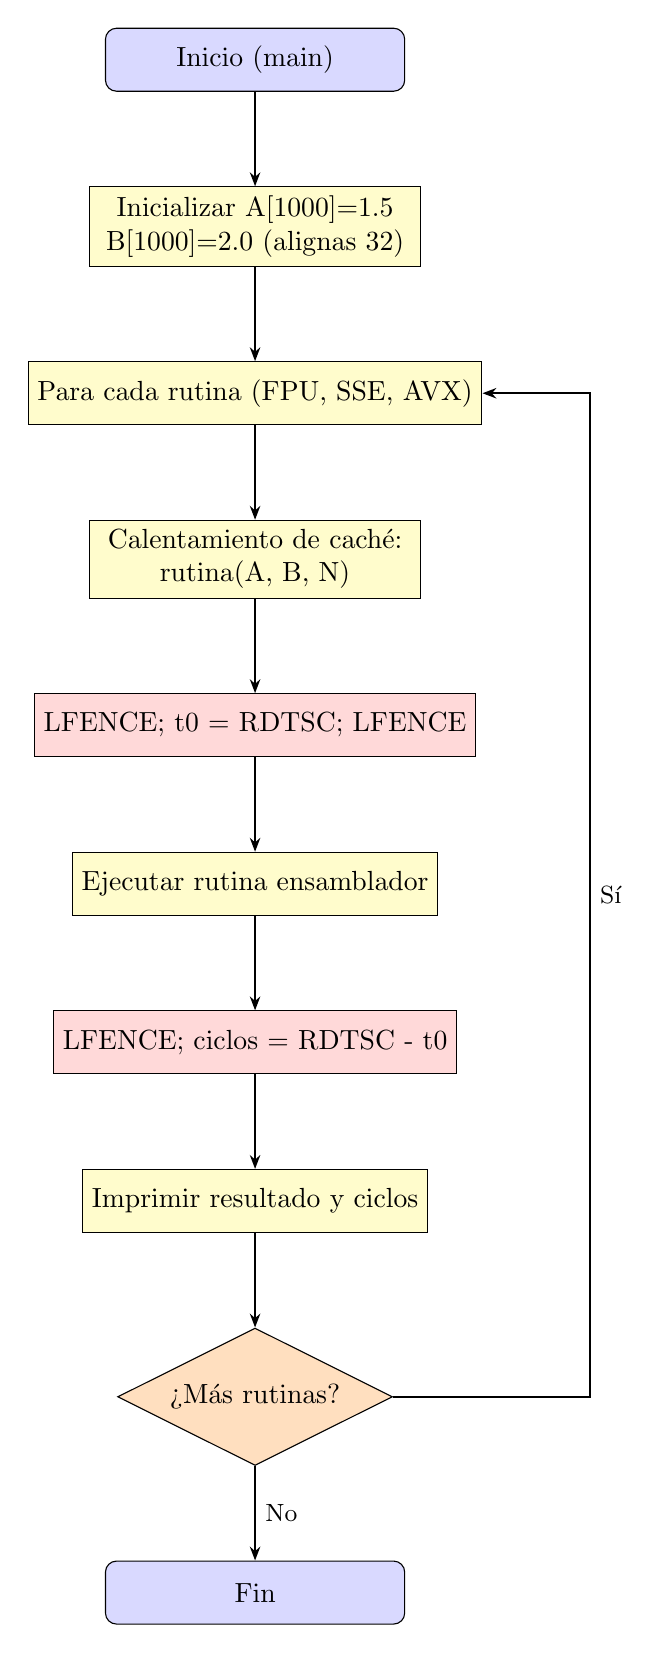
\begin{tikzpicture}[
            node distance=1.2cm and 2.2cm,
            startstop/.style={rectangle, rounded corners, draw=black, fill=blue!15,
                              minimum width=3.8cm, minimum height=0.8cm, align=center},
            process/.style  ={rectangle, draw=black, fill=yellow!20,
                              minimum width=4.2cm, minimum height=0.8cm, align=center},
            measure/.style  ={rectangle, draw=black, fill=red!15,
                              minimum width=4.2cm, minimum height=0.8cm, align=center},
            decision/.style ={diamond, draw=black, fill=orange!25,
                              minimum width=2.8cm, minimum height=0.8cm, align=center,
                              aspect=2},
            arrow/.style    ={-{Stealth[length=5pt]}, thick}
        ]
        \node[startstop] (inicio)  {Inicio (main)};
        \node[process, below=of inicio]  (init)    {Inicializar A[1000]=1.5\\B[1000]=2.0 (alignas 32)};
        \node[process, below=of init]    (loop)    {Para cada rutina (FPU, SSE, AVX)};
        \node[process, below=of loop]    (warm)    {Calentamiento de caché:\\rutina(A, B, N)};
        \node[measure, below=of warm]    (rdtsc1)  {LFENCE; t0 = RDTSC; LFENCE};
        \node[process, below=of rdtsc1]  (run)     {Ejecutar rutina ensamblador};
        \node[measure, below=of run]     (rdtsc2)  {LFENCE; ciclos = RDTSC - t0};
        \node[process, below=of rdtsc2]  (print)   {Imprimir resultado y ciclos};
        \node[decision, below=of print]  (more)    {¿Más rutinas?};
        \node[startstop, below=of more]  (fin)     {Fin};

        \draw[arrow] (inicio)  -- (init);
        \draw[arrow] (init)    -- (loop);
        \draw[arrow] (loop)    -- (warm);
        \draw[arrow] (warm)    -- (rdtsc1);
        \draw[arrow] (rdtsc1)  -- (run);
        \draw[arrow] (run)     -- (rdtsc2);
        \draw[arrow] (rdtsc2)  -- (print);
        \draw[arrow] (print)   -- (more);
        \draw[arrow] (more.east) -- ++(2.5,0) |- node[right, pos=0.25]{\small Sí} (loop.east);
        \draw[arrow] (more)    -- node[right]{\small No} (fin);
        \end{tikzpicture}
    }
    \caption{Diagrama de flujo de la medición de tiempos}
\end{figure}


% ============================================================
\section{Código fuente}

\subsection{Programa principal (main.cpp)}

El programa principal reserva los vectores con \texttt{alignas(32)} (requisito de AVX), los inicializa, y mide el costo de cada rutina con \texttt{RDTSC}+\texttt{LFENCE}. Para evitar repetir el bloque de medición, las tres rutinas se almacenan en un arreglo de punteros a función.

\begin{lstlisting}[language=CPP, caption={\texttt{main.cpp} — medición con RDTSC y LFENCE}]
#include <cstdio>
#include <intrin.h>

extern "C" float productoPunto_fpu(const float*, const float*, size_t);
extern "C" float productoPunto_sse(const float*, const float*, size_t);
extern "C" float productoPunto_avx(const float*, const float*, size_t);

int main() {
    alignas(32) static float A[1000];
    alignas(32) static float B[1000];

    for (int i = 0; i < 1000; i++) {
        A[i] = 1.5f;
        B[i] = 2.0f;
    }

    using Func = float(*)(const float*, const float*, size_t);
    Func rutinas[]        = { productoPunto_fpu, productoPunto_sse, productoPunto_avx };
    const char* nombres[] = { "FPU",             "SSE",             "AVX"             };

    printf("Calculando Producto Punto (N = 1000)\n");
    printf("--------------------------------------------------\n");

    for (int i = 0; i < 3; i++) {
        rutinas[i](A, B, 1000);                  // calentamiento

        _mm_lfence();
        unsigned __int64 inicio = __rdtsc();
        _mm_lfence();

        float res = rutinas[i](A, B, 1000);

        _mm_lfence();
        unsigned __int64 ciclos = __rdtsc() - inicio;

        printf("%s | Res: %.1f | Tiempo: %llu ciclos\n", nombres[i], res, ciclos);
    }
    return 0;
}
\end{lstlisting}

\subsection{Módulo ensamblador (tiempo.asm)}

El archivo \texttt{tiempo.asm} contiene las tres rutinas declaradas con \texttt{PUBLIC} para que el linker pueda resolverlas desde C++. Todas siguen la convención de llamadas Microsoft x64: \texttt{RCX}=primer puntero, \texttt{RDX}=segundo puntero, \texttt{R8}=dimensión, retorno en \texttt{XMM0}.

\begin{lstlisting}[language=MASM, caption={\texttt{productoPunto\_fpu} — versión FPU x87 (1 float por iteración)}]
productoPunto_fpu PROC
    xor  r9, r9                       ; i = 0
    fldz                              ; ST(0) = 0.0 (acumulador)
L1_fpu:
    cmp  r9, r8
    jge  L2_fpu
    fld  DWORD PTR [rcx + r9*4]       ; ST(0) = vecA[i]
    fmul DWORD PTR [rdx + r9*4]       ; ST(0) *= vecB[i]
    faddp st(1), st(0)                ; acum += ST(0); pop
    inc  r9
    jmp  L1_fpu
L2_fpu:
    sub  rsp, 8
    fstp DWORD PTR [rsp]              ; guarda ST(0) en pila
    movss xmm0, DWORD PTR [rsp]       ; copia a XMM0 (retorno)
    add  rsp, 8
    ret
productoPunto_fpu ENDP
\end{lstlisting}

\begin{lstlisting}[language=MASM, caption={\texttt{productoPunto\_sse} — versión SSE de 128 bits (4 floats por iteración)}]
productoPunto_sse PROC
    xorps xmm0, xmm0                  ; acumulador = (0, 0, 0, 0)
    xor   r9, r9
L1_sse:
    cmp  r9, r8
    jge  L2_sse
    movaps xmm1, XMMWORD PTR [rcx + r9*4]   ; carga 4 floats de vecA
    mulps  xmm1, XMMWORD PTR [rdx + r9*4]   ; *= 4 floats de vecB
    addps  xmm0, xmm1                       ; acumula 4 productos
    add  r9, 4
    jmp  L1_sse
L2_sse:
    haddps xmm0, xmm0                       ; reducción horizontal
    haddps xmm0, xmm0                       ; resultado escalar en XMM0
    ret
productoPunto_sse ENDP
\end{lstlisting}

\begin{lstlisting}[language=MASM, caption={\texttt{productoPunto\_avx} — versión AVX de 256 bits (8 floats por iteración)}]
productoPunto_avx PROC
    vxorps ymm0, ymm0, ymm0           ; acumulador YMM = 8 ceros
    xor    r9, r9
L1_avx:
    cmp  r9, r8
    jge  L2_avx
    vmovaps ymm1, YMMWORD PTR [rcx + r9*4]      ; carga 8 floats de vecA
    vmulps  ymm1, ymm1, YMMWORD PTR [rdx + r9*4] ; *= 8 floats de vecB
    vaddps  ymm0, ymm0, ymm1                     ; acumula 8 productos
    add  r9, 8
    jmp  L1_avx
L2_avx:
    vextractf128 xmm1, ymm0, 1        ; reduce 256 -> 128 bits
    vaddps  xmm0, xmm0, xmm1
    vhaddps xmm0, xmm0, xmm0          ; reducción horizontal
    vhaddps xmm0, xmm0, xmm0
    vzeroupper                        ; limpia estado AVX
    ret
productoPunto_avx ENDP
\end{lstlisting}

% ============================================================
\section{Instrucciones x86/x64 utilizadas}

\subsection{FPU x87}

\begin{table}[H]
    \centering
    \begin{tabular}{@{}lp{10cm}@{}}
        \toprule
        \textbf{Instrucción} & \textbf{Operación} \\
        \midrule
        \texttt{FLDZ}  & Carga \texttt{0.0} al tope de la pila FPU. \\
        \texttt{FLD}   & Carga un \texttt{float} (4 bytes) desde memoria a \texttt{ST(0)}. \\
        \texttt{FMUL}  & Multiplica \texttt{ST(0)} por un operando de memoria. \\
        \texttt{FADDP} & Suma \texttt{ST(0)} a \texttt{ST(1)} y hace \textit{pop}. \\
        \texttt{FSTP}  & Guarda \texttt{ST(0)} en memoria y hace \textit{pop}. \\
        \texttt{MOVSS} & Copia un \texttt{float} (\textit{scalar single}) entre memoria y XMM. \\
        \bottomrule
    \end{tabular}
    \caption{Instrucciones x87 usadas en \texttt{productoPunto\_fpu}}
\end{table}

\subsection{SSE (128 bits, 4 floats empaquetados)}

\begin{table}[H]
    \centering
    \begin{tabular}{@{}lp{10cm}@{}}
        \toprule
        \textbf{Instrucción} & \textbf{Operación} \\
        \midrule
        \texttt{XORPS}  & XOR empaquetado: limpia los 128 bits de un registro XMM. \\
        \texttt{MOVAPS} & \textit{Move Aligned Packed Single}: carga 4 floats alineados desde memoria. \\
        \texttt{MULPS}  & Multiplica 4 floats por 4 floats (elemento a elemento). \\
        \texttt{ADDPS}  & Suma 4 floats con 4 floats. \\
        \texttt{HADDPS} & Suma horizontal: suma pares adyacentes dentro del registro XMM. \\
        \bottomrule
    \end{tabular}
    \caption{Instrucciones SSE usadas en \texttt{productoPunto\_sse}}
\end{table}

\subsection{AVX (256 bits, 8 floats empaquetados)}

\begin{table}[H]
    \centering
    \begin{tabular}{@{}lp{10cm}@{}}
        \toprule
        \textbf{Instrucción} & \textbf{Operación} \\
        \midrule
        \texttt{VXORPS}       & Versión AVX de XOR (limpia un registro YMM completo). \\
        \texttt{VMOVAPS}      & Carga 8 floats alineados a 32 bytes desde memoria. \\
        \texttt{VMULPS}       & Multiplica 8 floats por 8 floats. \\
        \texttt{VADDPS}       & Suma 8 floats con 8 floats. \\
        \texttt{VEXTRACTF128} & Extrae la mitad alta de un YMM a un XMM (reducción 256$\to$128). \\
        \texttt{VHADDPS}      & Suma horizontal AVX. \\
        \texttt{VZEROUPPER}   & Limpia la mitad alta de los registros YMM (evita penalización AVX$\to$SSE). \\
        \bottomrule
    \end{tabular}
    \caption{Instrucciones AVX usadas en \texttt{productoPunto\_avx}}
\end{table}

\subsection{Instrumentación de tiempo}

\begin{table}[H]
    \centering
    \begin{tabular}{@{}lp{10cm}@{}}
        \toprule
        \textbf{Instrucción} & \textbf{Operación} \\
        \midrule
        \texttt{RDTSC}  & \textit{Read Time-Stamp Counter}: devuelve en \texttt{EDX:EAX} el contador de ciclos del procesador desde su último \textit{reset}. \\
        \texttt{LFENCE} & \textit{Load Fence}: serializa la ejecución; impide que las cargas posteriores se ejecuten antes de que las anteriores terminen. \\
        \bottomrule
    \end{tabular}
    \caption{Instrucciones de medición usadas en \texttt{main.cpp} a través de intrínsecos}
\end{table}

% ============================================================
\section{El rol de los registros}

\subsection{Convención de llamadas Microsoft x64}

A diferencia de la \textit{cdecl} de 32 bits (parámetros en la pila), en x64 los primeros cuatro argumentos enteros viajan en registros. Esta práctica solo usa los tres primeros:

\begin{table}[H]
    \centering
    \begin{tabular}{@{}llp{6.5cm}@{}}
        \toprule
        \textbf{Registro} & \textbf{Parámetro} & \textbf{Descripción} \\
        \midrule
        \texttt{RCX} & \texttt{const float* vecA} & Puntero al primer vector. \\
        \texttt{RDX} & \texttt{const float* vecB} & Puntero al segundo vector. \\
        \texttt{R8}  & \texttt{size\_t N}         & Dimensión de los vectores (1000). \\
        \texttt{XMM0} & retorno                   & La parte baja contiene el \texttt{float} resultado. \\
        \bottomrule
    \end{tabular}
    \caption{Mapa de parámetros para la convención Microsoft x64}
\end{table}

\subsection{Registros internos de las rutinas}

\begin{table}[H]
    \centering
    \begin{tabular}{@{}llp{7cm}@{}}
        \toprule
        \textbf{Registro} & \textbf{Rutina} & \textbf{Rol} \\
        \midrule
        \texttt{R9}            & las tres   & Índice de iteración \texttt{i}. \\
        \texttt{ST(0), ST(1)}  & FPU        & Acumulador y operando temporal en la pila FPU. \\
        \texttt{XMM0}          & SSE        & Acumulador empaquetado de 4 floats. \\
        \texttt{XMM1}          & SSE        & Carga temporal de 4 floats desde memoria. \\
        \texttt{YMM0}          & AVX        & Acumulador empaquetado de 8 floats. \\
        \texttt{YMM1}          & AVX        & Carga temporal de 8 floats. \\
        \bottomrule
    \end{tabular}
    \caption{Registros internos usados por cada rutina}
\end{table}

% ============================================================
\section{Comparación teórica}

Cada rutina realiza la misma cantidad de \textbf{trabajo lógico} (1000 multiplicaciones y 1000 sumas), pero el \textbf{número de iteraciones} del bucle difiere:

\begin{table}[H]
    \centering
    \begin{tabular}{@{}lccc@{}}
        \toprule
        \textbf{Rutina} & \textbf{Floats/iter.} & \textbf{Iteraciones (N=1000)} & \textbf{Speedup teórico} \\
        \midrule
        FPU x87 & 1 & 1000 & $1\times$ (referencia) \\
        SSE     & 4 & 250  & $4\times$ \\
        AVX     & 8 & 125  & $8\times$ \\
        \bottomrule
    \end{tabular}
    \caption{Iteraciones y \textit{speedup} teórico para $N=1000$}
\end{table}

En la práctica, el \textit{speedup} medido es \textbf{menor} que el teórico por:
\begin{itemize}
    \item Latencia de las propias instrucciones SIMD (algunas son más caras que su contraparte escalar).
    \item Costo fijo de la \textbf{reducción horizontal} (\texttt{HADDPS}, \texttt{VEXTRACTF128}).
    \item Acceso a memoria limitado por el ancho de banda L1.
    \item Sobrecarga del prólogo, epílogo y \texttt{vzeroupper}.
\end{itemize}

% ============================================================
\section{Ejemplo de ejecución}

% ============================================================
% INSTRUCCIONES PARA OBTENER LAS CAPTURAS DE PANTALLA
% ============================================================
%
% CAPTURA 1: imagenes/consola_ejecucion.png
% -----------------------------------------
% 1) Abrir Practica07_TiemposEjecucion.slnx en Visual Studio.
% 2) En la barra superior elegir "Release | x64"
%    (en Debug los ciclos son mucho mayores y poco representativos).
% 3) Compilar con Ctrl+Shift+B y ejecutar con Ctrl+F5 (sin depurar).
% 4) Esperar a que aparezcan las 3 líneas: FPU, SSE, AVX con sus ciclos.
% 5) Hacer captura de la ventana de consola completa (Alt+ImprPant).
% 6) Guardar como  documentacion/imagenes/consola_ejecucion.png
%
% CAPTURA 2: imagenes/registros_avx.png
% --------------------------------------
% 1) Abrir Practica07_TiemposEjecucion.slnx, configuración Debug | x64.
% 2) En tiempo.asm, poner un breakpoint en la línea "vaddps ymm0, ymm0, ymm1"
%    dentro de productoPunto_avx (clic en margen izquierdo).
% 3) Pulsar F5 para iniciar la depuración.
% 4) Cuando se detenga en el breakpoint, abrir:
%    Debug -> Windows -> Registers
% 5) En la ventana de Registers hacer clic derecho y activar el grupo
%    "SSE2"  (muestra XMM0..XMM15) y "AVX" (muestra YMM0..YMM15).
% 6) Pulsar F10 varias veces para observar cómo cambia YMM0 al acumular.
% 7) Hacer captura de la ventana de Registers (Alt+ImprPant sobre VS).
% 8) Guardar como  documentacion/imagenes/registros_avx.png
%
% CAPTURA 3: imagenes/comparacion_ciclos.png  (opcional, gráfico)
% ---------------------------------------------------------------
% 1) Ejecutar el programa al menos 5 veces (como en CAPTURA 1) y
%    anotar los ciclos de FPU, SSE y AVX.
% 2) En Excel/LibreOffice/Google Sheets construir una tabla con
%    las 5 mediciones por rutina y calcular el promedio.
% 3) Generar un gráfico de barras horizontales: en el eje Y las
%    rutinas (FPU, SSE, AVX); en el eje X los ciclos promedio.
% 4) Exportar el gráfico como PNG (clic derecho -> Guardar como imagen).
% 5) Guardar como  documentacion/imagenes/comparacion_ciclos.png
% ============================================================

Tras compilar en \textbf{Release | x64} y ejecutar el programa, la consola muestra el resultado de las tres rutinas y los ciclos consumidos por cada una. El resultado debe ser \texttt{3000.0} en las tres (correctitud), y los ciclos deben respetar la jerarquía \texttt{FPU > SSE > AVX}:

\begin{figure}[H]
    \centering
    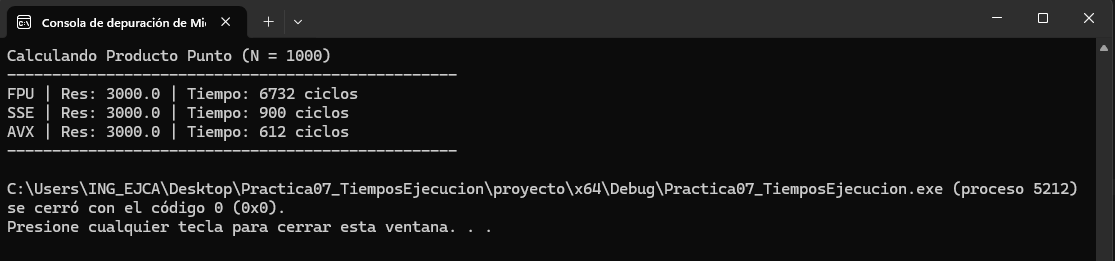
\includegraphics[width=0.9\textwidth]{imagenes/consola_ejecucion.png}
    \caption{Salida en consola del programa para $N=1000$ con $A_i=1.5$ y $B_i=2.0$. Las tres rutinas devuelven \texttt{3000.0}; los ciclos descienden de FPU a SSE a AVX, mostrando la ganancia del paralelismo SIMD.}
    \label{fig:consola_p07}
\end{figure}

\subsection{Inspección de los registros AVX durante la ejecución}

Para verificar que los registros YMM contienen los 8 floats esperados, se coloca un \textit{breakpoint} dentro del bucle de \texttt{productoPunto\_avx} y se observa el contenido de \texttt{YMM0} (acumulador) y \texttt{YMM1} (carga temporal) en la ventana \textit{Registers} de Visual Studio:

\begin{figure}[H]
    \centering
    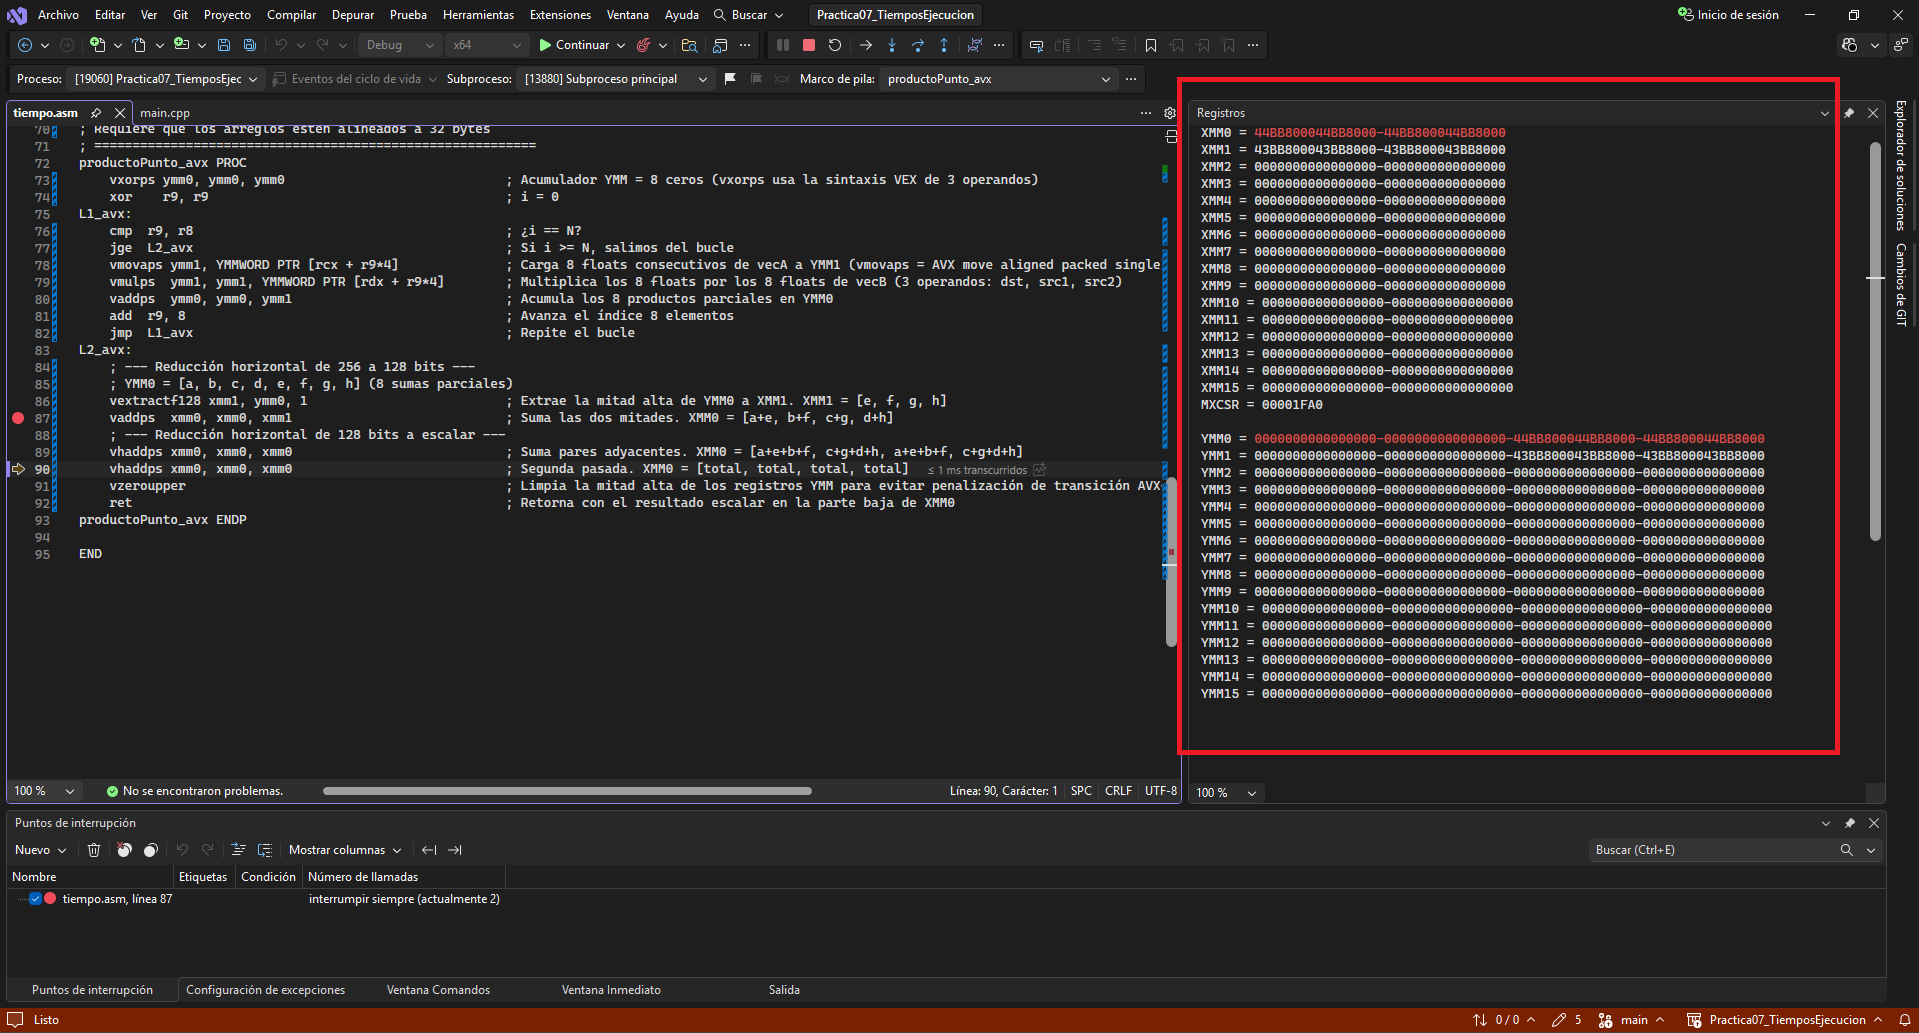
\includegraphics[width=0.9\textwidth]{imagenes/registros_avx.png}
    \caption{Ventana \textit{Registers} de Visual Studio durante el bucle AVX: \texttt{YMM1} contiene 8 productos $1.5 \times 2.0 = 3.0$ y \texttt{YMM0} acumula los productos parciales en sus 8 carriles.}
    \label{fig:registros_avx}
\end{figure}

\subsection{Comparación gráfica de ciclos}

Al ejecutar el programa varias veces y promediar los ciclos, se observa con claridad que AVX es el más rápido, seguido por SSE y, en último lugar, la FPU:

\begin{figure}[H]
    \centering
    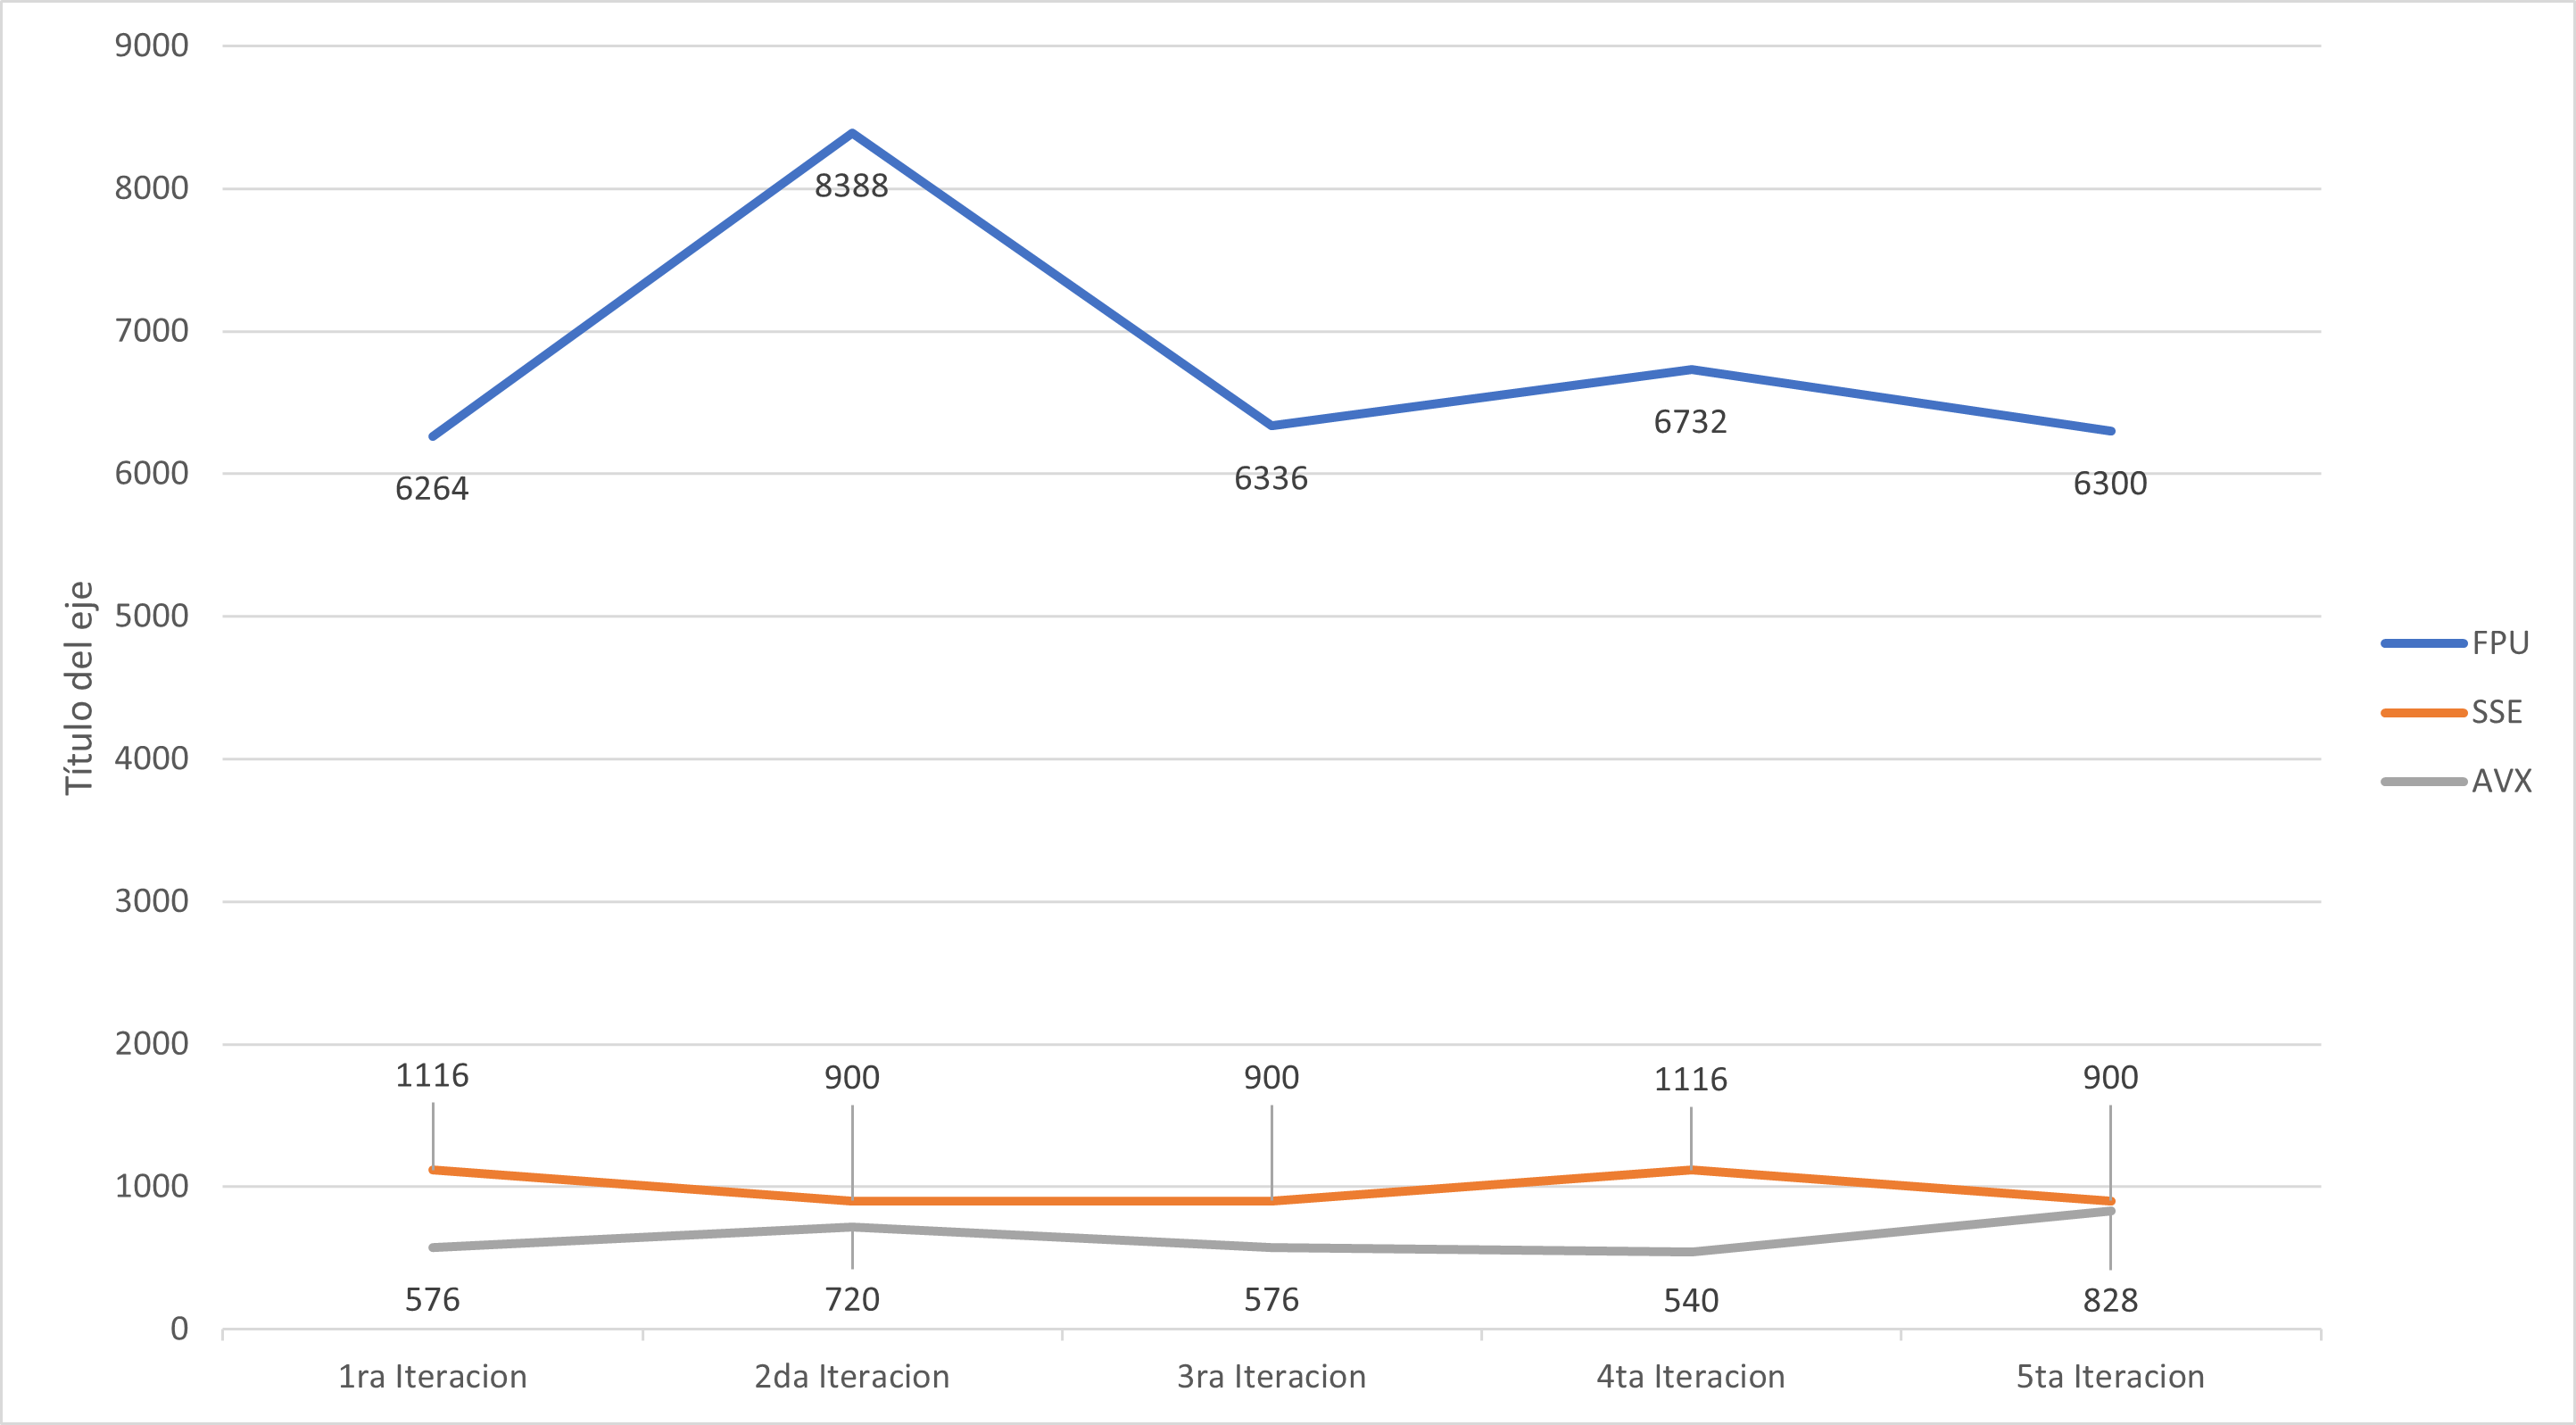
\includegraphics[width=0.9\textwidth]{imagenes/comparacion_ciclos.png}
    \caption{Comparación de ciclos promedio para las tres rutinas (5 ejecuciones, $N=1000$). El paralelismo SIMD reduce sustancialmente el costo del producto punto.}
    \label{fig:comparacion}
\end{figure}

% ============================================================
\section{Repositorio GitHub}

\url{https://github.com/7mo-ArquitecturaComputadoras/Practica07_TiemposEjecucion}

% ============================================================
\section{Conclusiones}

\begin{itemize}
    \item La comparación FPU vs SSE vs AVX demuestra en términos cuantitativos el valor del \textbf{paralelismo a nivel de datos}: una sola instrucción \texttt{VMULPS} sustituye a ocho \texttt{FMUL} consecutivos, lo que reduce drásticamente el número de instrucciones decodificadas, despachadas y retiradas por el procesador.

    \item El uso de \texttt{RDTSC} entre \texttt{LFENCE} es esencial para medir con precisión: sin las barreras, el procesador puede mover instrucciones a través del \texttt{RDTSC} y producir lecturas inconsistentes. El calentamiento previo de la caché L1 también es necesario, pues la primera invocación incluye el costo de los fallos de caché.

    \item La \textbf{reducción horizontal} (\texttt{HADDPS}, \texttt{VEXTRACTF128} + \texttt{VHADDPS}) es un sobrecosto inherente a SIMD: el acumulador termina con varios valores parciales que es necesario sumar entre sí. Para vectores grandes este costo se amortiza, pero para vectores pequeños puede dominar.

    \item La instrucción \texttt{VZEROUPPER} al final de la rutina AVX evita la \textbf{penalización de transición} entre los modos AVX y SSE: si se omitiera, una llamada posterior a código SSE puro sufriría una latencia adicional de varios cientos de ciclos en algunas microarquitecturas.

    \item La alineación de memoria a 32 bytes (\texttt{alignas(32)}) es \textbf{obligatoria} para las cargas alineadas \texttt{VMOVAPS}; usar \texttt{VMOVUPS} (sin alineación) habría permitido tolerar arreglos mal alineados, pero a costa de microoperaciones extra en algunos procesadores. La elección refleja un principio común en programación SIMD: si tienes control sobre los datos, alíñalos.
\end{itemize}

\end{document}
